%%%%%%%%%%%%%%%%%%%%%%%%%%%%%%%%%%%%%%%%%
% baposter Portrait Poster
% LaTeX Template
% Version 1.0 (15/5/13)
%
% Created by:
% Brian Amberg (baposter@brian-amberg.de)
%
% This template has been downloaded from:
% http://www.LaTeXTemplates.com
%
% License:
% CC BY-NC-SA 3.0 (http://creativecommons.org/licenses/by-nc-sa/3.0/)
%
%%%%%%%%%%%%%%%%%%%%%%%%%%%%%%%%%%%%%%%%%

%----------------------------------------------------------------------------------------
%	PACKAGES AND OTHER DOCUMENT CONFIGURATIONS
%----------------------------------------------------------------------------------------

\documentclass[a0paper,portrait]{baposter}

\usepackage[font=small,labelfont=bf]{caption} % Required for specifying captions to tables and figures
\usepackage{booktabs} % Horizontal rules in tables
\usepackage{relsize} % Used for making text smaller in some places

\graphicspath{{figures/}} % Directory in which figures are stored

\definecolor{bordercol}{RGB}{40,40,40} % Border color of content boxes
\definecolor{headercol1}{RGB}{186,215,230} % Background color for the header in the content boxes (left side)
\definecolor{headercol2}{RGB}{80,80,80} % Background color for the header in the content boxes (right side)
\definecolor{headerfontcol}{RGB}{0,0,0} % Text color for the header text in the content boxes
\definecolor{boxcolor}{RGB}{255,255,255} % Background color for the content in the content boxes

\begin{document}

\background{ % Set the background to an image (background.pdf)

}

\begin{poster}{
grid=false,
borderColor=bordercol, % Border color of content boxes
headerColorOne=headercol1, % Background color for the header in the content boxes (left side)
headerColorTwo=headercol1, % Background color for the header in the content boxes (right side)
headerFontColor=headerfontcol, % Text color for the header text in the content boxes
boxColorOne=boxcolor, % Background color for the content in the content boxes
headershape=roundedright, % Specify the rounded corner in the content box headers
headerfont=\Large\sf\bf, % Font modifiers for the text in the content box headers
textborder=rectangle,
background=user,
headerborder=open, % Change to closed for a line under the content box headers
boxshade=plain
}
{}
%
%----------------------------------------------------------------------------------------
%	TITLE AND AUTHOR NAME
%----------------------------------------------------------------------------------------
%
{\sf\bf MoCA : Tool for Motif Conservation Analysis} % Poster title
{\vspace{1em} Saket Choudhary, Anton Valouev\\ % Author names
{\smaller {skchoudh, valouev}@uni.edu}} % Author email addresses
%{
\includegraphics[scale=0.3]{usclogo}} % University/lab logo

%----------------------------------------------------------------------------------------
%	INTRODUCTION
%----------------------------------------------------------------------------------------

\headerbox{Introduction}{name=introduction,column=0,row=0, span=3}{


}

%----------------------------------------------------------------------------------------
%	MATERIALS AND METHODS
%----------------------------------------------------------------------------------------

\headerbox{Materials and Methods}{name=methods,column=0,below=introduction}{

\begin{description}
\item[ER1] Sed a orci non ipsum posuere placerat. Nunc in mi augue, a adipiscing massa. Donec dapibus gravida odio, condimentum convallis urna.\item[ER2] Nullam sagittis cursus neque, sit amet mollis elit auctor in. Etiam sed lectus a nulla rhoncus interdum a tempus nunc. Sed at eleifend purus.
\end{description}

Nullam sollicitudin lobortis urna quis varius. Nullam sagittis blandit diam, $DN = G_t(V_t,E_t)$, risus $E_t \subseteq V_t \times V_t$ ($\forall t \geq 0$). vel tortor justo, $G_0$, quis malesuada lorem.


}

%----------------------------------------------------------------------------------------
%	CONCLUSION
%----------------------------------------------------------------------------------------

\headerbox{Conclusion}{name=conclusion,column=0,below=methods}{


}

%----------------------------------------------------------------------------------------
%	REFERENCES
%----------------------------------------------------------------------------------------

\headerbox{References}{name=references,column=0,below=conclusion}{

\smaller % Reduce the font size in this block
\renewcommand{\section}[2]{\vskip 0.05em} % Get rid of the default "References" section title
\nocite{*} % Insert publications even if they are not cited in the poster

\bibliographystyle{unsrt}
\bibliography{sample} % Use sample.bib as the bibliography file
}

%----------------------------------------------------------------------------------------
%	ACKNOWLEDGEMENTS
%----------------------------------------------------------------------------------------

% \headerbox{Acknowledgements}{name=acknowledgements,column=0,below=references, above=bottom}{

% \smaller % Reduce the font size in this block
% Fusce mattis tellus ac odio imperdiet lobortis. Cum sociis natoque penatibus et magnis dis parturient montes, nascetur ridiculus mus. Phasellus commodo blandit euismod. Ut porttitor cursus magna. Mauris adipiscing pellentesque ipsum nec facilisis. Cras ornare bibendum bibendum. Ut a elit purus, vel adipiscing.
% } 



%------------------------------------------------



%----------------------------------------------------------------------------------------
%	RESULTS
%----------------------------------------------------------------------------------------

\headerbox{Results Heading 2}{name=results2,span=2,column=1,below=introduction,above=bottom}{ % To reduce this block to 1 column width, remove 'span=2'



%------------------------------------------------

% \begin{center}
% 
\includegraphics[width=0.49\linewidth]{placeholder}
% 
\includegraphics[width=0.49\linewidth]{placeholder}
% \captionof{figure}{Figure caption 1 (left); Figure caption 2 (right)}
% \end{center}

%------------------------------------------------



%------------------------------------------------

\begin{center}
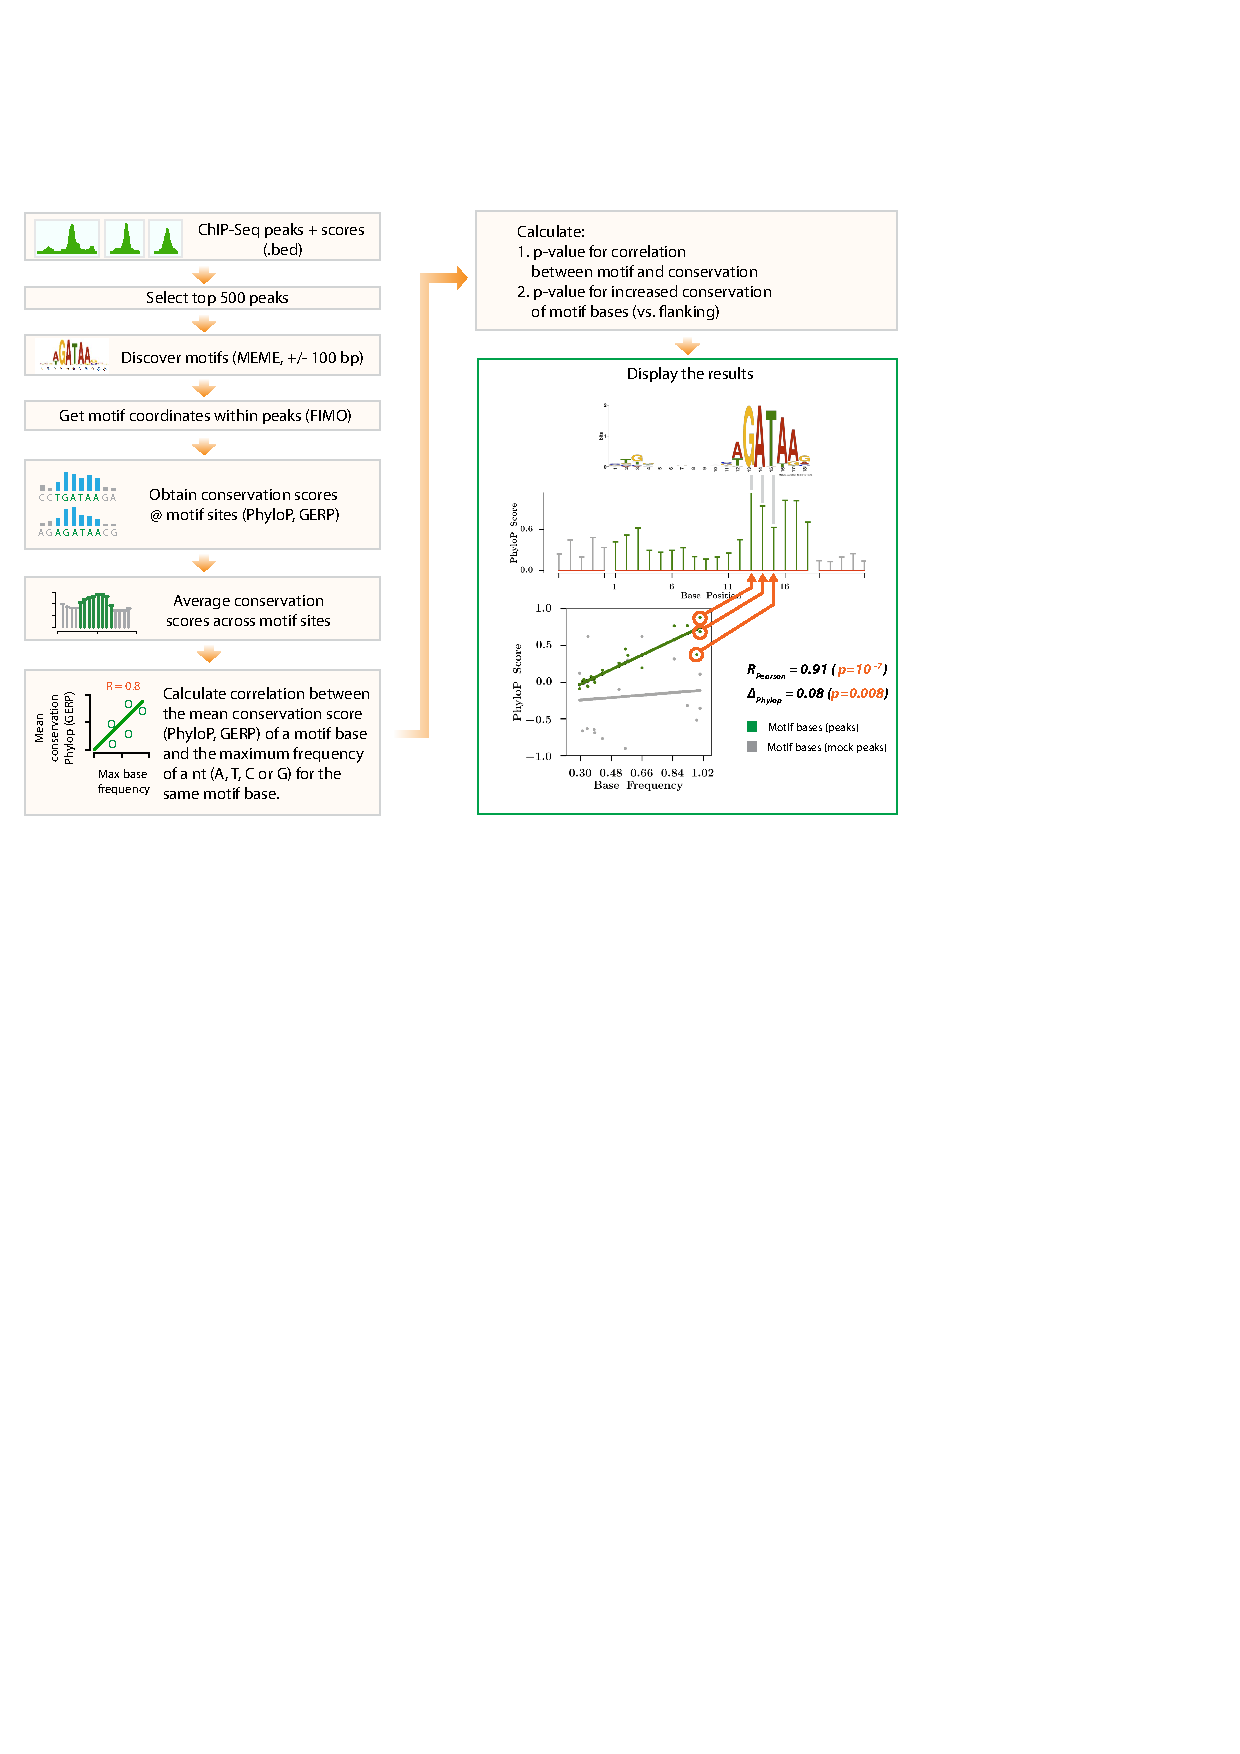
\includegraphics[width=\linewidth]{workflow}
\captionof{figure}{MoCA Workflow}
\end{center}

%------------------------------------------------


}

%----------------------------------------------------------------------------------------

\end{poster}

\end{document}